\section{Free Body Diagrams}

\blue{Insert the same content here as from the TAM212 Reference Pages (Free Body Diagrams - the top introduction section). Note that if you try to click on the link to "Free Body Diagrams" from the TAM 210 reference page it doesn't work. You have to go into the TAM 212 reference page to access Free Body Diagrams. }

\subsection{Pulley Idealizations}

In this course we assume that a pulley is frictionless, meaning that the magnitude of the tensile force of the rope on either side of a pulley will be the same. 

\[{T_1} = {T_2}\]

\begin{figure*}[!h]
\centering
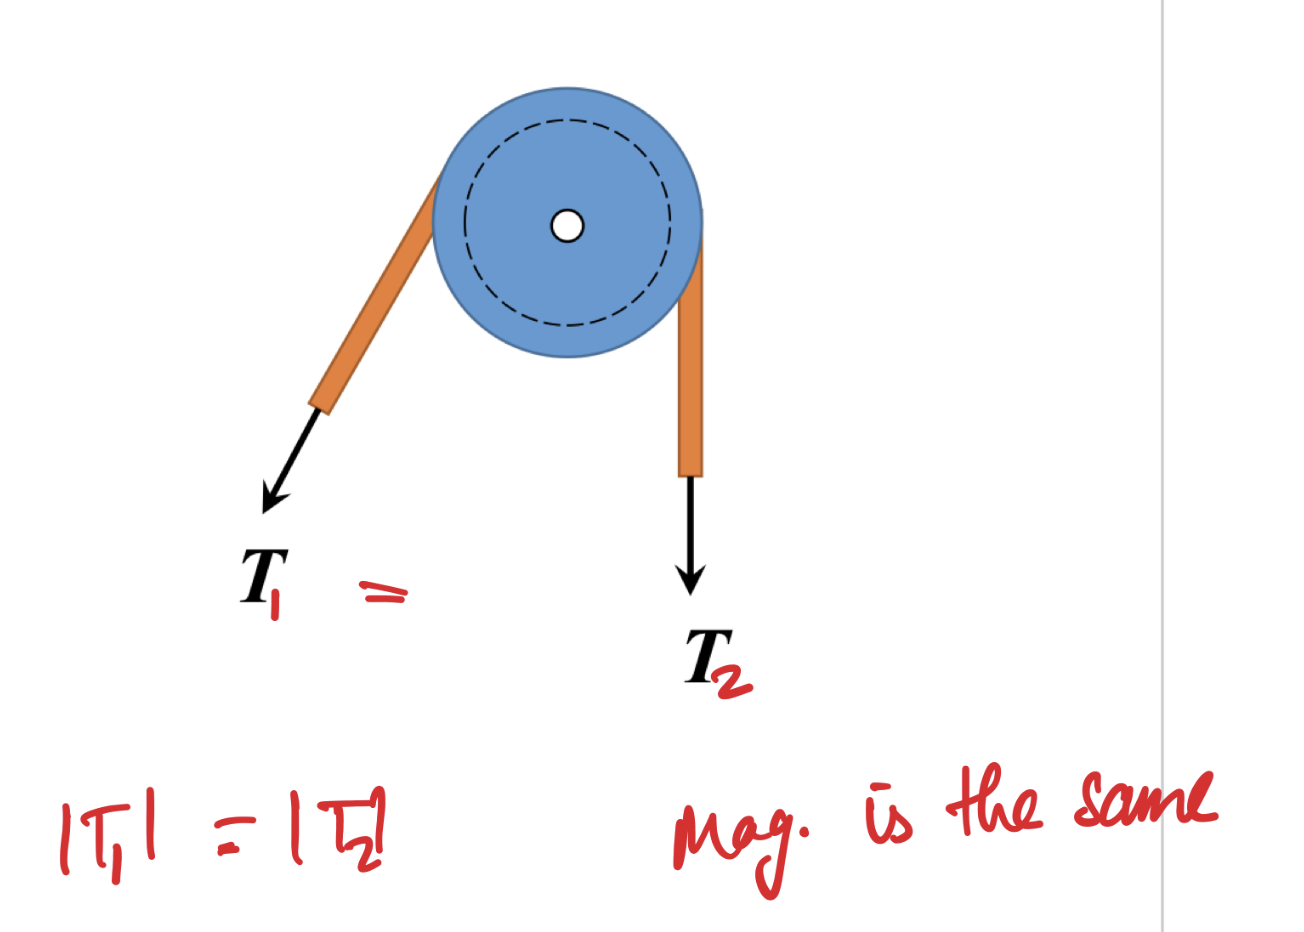
\includegraphics[angle=0, width=3in]{FBDFigures/PulleyAssumptions.png}
\vspace{-2mm}
\caption{\small \blue{Taken from TAM 210 Lecture 5 - Slide 6}}
\vspace{-3mm}
\label{Fig:PulleyAsusmptions}
\end{figure*}

\subsection{Spring Idealizations}

In this course, we assume springs are linearly elastic, which means that the force (tension) in the spring is linearly proportional to the extension of the spring ($s$) through the spring constant, $k$.

\[{F} = {k*s}\]

\[{s} = {l-l_0}\]

\begin{figure*}[!h]
\centering
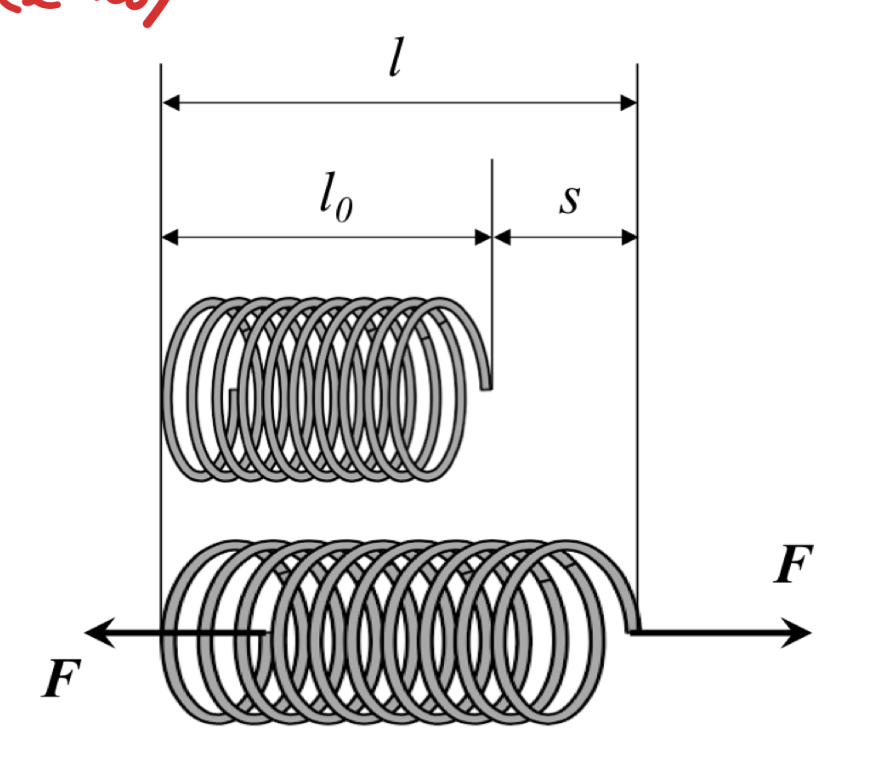
\includegraphics[angle=0, width=2in]{FBDFigures/SpringAssumptions.png}
\vspace{-2mm}
\caption{\small \blue{Taken from TAM 210 Lecture 5 - Slide 7. Make this picture and put it next to a stress-strain curve with the straight linear elastic line and the slope as k.}}
\vspace{-3mm}
\label{Fig:SpringAssumptions}
\end{figure*}

\subsection{Smooth Surface Idealizations}

If a surface is described as "smooth", we assume that there is no frictional force on the surface. Therefore, any force applied by the surface is normal to the surface. 

\begin{figure*}[!h]
\centering
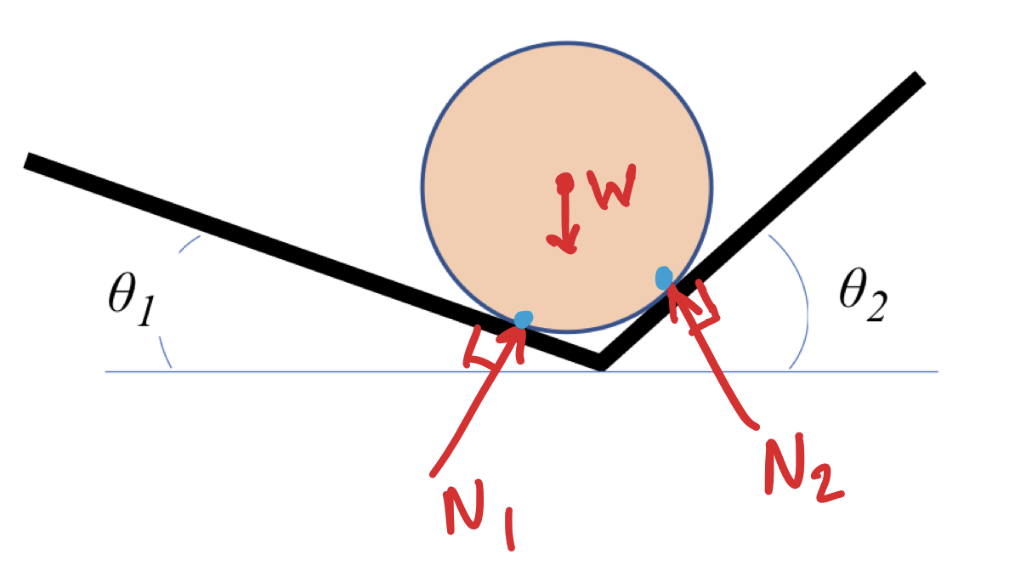
\includegraphics[angle=0, width=3in]{FBDFigures/SmoothAssumptions.png}
\vspace{-2mm}
\caption{\small \blue{Taken from TAM 210 Lecture 5 - Slide 8. This could become an interactive image eventually where the angles of the surfaces are changed by the user and then the reaction forces are also changing.}}
\vspace{-3mm}
\label{Fig:SmoothAssumptions}
\end{figure*}

%\subsection{\red{Equivalent force systems}}
%lecture 10